\documentclass[12pt, a4paper]{article}
\usepackage[utf8]{inputenc}
\usepackage[T2A]{fontenc}
\usepackage{indentfirst, setspace}
\usepackage{tabularx, multirow}
\usepackage[normalem]{ulem}
\usepackage[style=russian]{csquotes}
\usepackage[english,russian]{babel}
\usepackage{hyperref}
\usepackage{ragged2e}
\usepackage{caption}
\usepackage{wrapfig}
\usepackage{amsmath}
\usepackage{tikz}
\makeatletter
\def\@biblabel#1{#1. }
\makeatother
\captionsetup{labelsep=endash}
\usepackage{listings}
\linespread{1.3}
\lstset{
  language=C++,
  basicstyle=\ttfamily\small,
  keywordstyle=\color{blue},
  breaklines=true,
  commentstyle=\color{green},
  stringstyle=\color{red},
  extendedchars=\true,
  showstringspaces=false,
  keepspaces=true,
}

\usepackage[left=2cm,right=2cm,
    top=2cm,bottom=2cm,bindingoffset=0cm]{geometry}\begin{document}
\begin{titlepage}
     \fontsize{12}{12}\selectfont

  {\centering

   \begin{bf}

    \begin{wrapfigure}{l}{10mm}
        
\includegraphics[width=17mm]{photo_2023-12-20.jpeg}
    \end{wrapfigure}


    \noindent Министерство науки и высшего образования Российской Федерации

    \noindent Федеральное государственное бюджетное образовательное учреждение высшего образования

    \noindent \enquote{Московский государственный технический университет

     \noindent имени Н.Э. Баумана

     \noindent (национальный исследовательский университет)}

    \noindent (МГТУ им. Н.Э. Баумана)

   \end{bf}
  }

  \vspace{0.4cm}

  {\setstretch{0.1}
   \noindent\rule{\textwidth}{1mm}
   \noindent\rule{\textwidth}{0.5mm}

  }

  \fontsize{14}{21}\selectfont

  \noindent\begin{tabularx}{\textwidth}{l >{\centering\arraybackslash}X}
   ФАКУЛЬТЕТ & \flqq Фундаментальные Науки\frqq \\ \cline{2-2}

   КАФЕДРА & ФН-12 \flqq Математическое моделирование\frqq \\ \cline{2-2}
  \end{tabularx}

  \vspace{1cm}


  \begin{center}
   \begin{bf}

    \fontsize{24}{36}\selectfont
    ОТЧЕТ

    \fontsize{20}{30}\selectfont
    ПО ЛАБОРАТОРНОЙ РАБОТЕ НА ТЕМУ:

    АВЛ-дерево

   \end{bf}
  \end{center}

  \fontsize{14}{21}\selectfont
  \vspace{5cm}


  \noindent\begin{tabularx}{\textwidth}{ X >{\centering}p{4cm} p{1cm} c }
   Студент: & & & Мациевский И. М. \\ \cline{2-2} \cline{4-4}
   & \fontsize{10}{15}\selectfont дата, подпись & & \fontsize{10}{15}\selectfont Ф.И.О. \\
   Преподаватель: & & & Волкова Л. Л.\\ \cline{2-2} \cline{4-4}
   & \fontsize{10}{15}\selectfont дата, подпись & & \fontsize{10}{15}\selectfont Ф.И.О.
   \end{tabularx}

  \vspace{\fill}

  \begin{center}
   \it{Москва}, 2023
  \end{center}

  \thispagestyle{empty}
\end{titlepage}\newpage
\tableofcontents
\newpage
\section*{Введение}
\addcontentsline{toc}{section}{Введение}
\justifying
\textbf{Цель лабораторной работы}: описать структуру 
данных АВЛ-дерева.

Для достижения поставленной цели требуется решить следующие 
\textbf{задачи}.
\begin{enumerate}
\item Описать алгоритмы добавления и удаления 
элемента, поиска элемента в дереве, балансировки дерева.
\item Разработать программу, предоставляющую пользователю выбор пункта 
меню, отображающую меню в цикле с постусловием, реализующую все описанные 
алгоритмы.
\end{enumerate}
\newpage
\section{Аналитическая часть}
\textbf{АВЛ-дерево ---} это сбалансированное двоичное дерево поиска, в 
котором поддерживается следующее свойство: для каждой его вершины высота её 
двух поддеревьев различается не более чем на 1.
Преимущество таких деревьев в том, что они поддерживают логарифмическое 
время поиска, в отличие обычных деревьев, в которых в худшем случае поиск
проходит за $O(N)$.

Для описания структуры АВЛ-дерева используется класс $AVLTree$.
Для работы с этой структурой реализованы следующие методы: поиск высоты 
дерева, нахождение разницы между левым и правым поддеревом, поворот направо
и налево для балансировки дерева при добавлении нового элемента, добавление
элемента, нахождение узла с минимальным ключом, удаление узла, поиск узла,
вывод меню на экран, вывод дерева на экран, вывод указателя на корень 
дерева.
\newpage
\section{Конструкторская часть}
\textbf{Реализованные методы и функции}
\begin{enumerate}
	\item $Height$ возвращает $0$, если дерево пусто, иначе его высоту.
	\item $BalanceFactor$ подсчитывает разницу между поддеревьями одного
	узла и возвращает ее.
	\item $rotateRight$ выполняет операцию правого вращения, для этого 
	сначала сохраняется указатель на левого потомка($x$) и правое поддерево
	($T2$) данного узла $y$, затем происходит поворот: $x$ становится 
	узлом, $y$ становится левым поддеревом, а $T2$ правым поддеревом, 
	возвращается указатель на новый корень поддерева.
	\item $rotateLeft$ выполняет операцию левого вращения, для этого 
	сначала сохраняется указатель на правого потомка($y$) и левое поддерево
	($T2$) данного узла $x$, затем происходит поворот: $y$ становится 
	узлом, $x$ становится левым поддеревом, а $T2$ правым поддеревом, 
	возвращается указатель на новый корень поддерева.
	\item $balance$ выполняет балансировку дерева, начиная с заданного узла
	проверяет, нарушается ли баланс в узле, если да, применяет 
	соответствующие вращения для восстановления баланса.
	\begin{enumerate}
		\item Если узел $node$ равен $nullptr$, то возвращается $nullptr$. 
		Дерево пусто и балансировка не требуется.
		\item Высота узла $node$ обновляется, исходя из максимальных высот 
		его левого и правого поддеревьев.
		\item Вычисляется фактор баланса для узла $node$, который 
		представляет собой разницу между высотой правого и левого 
		поддеревьев.
		\item Если фактор баланса больше 1 и фактор баланса левого 
		поддерева $node->left$ неотрицателен, то происходит правое вращение 
		($rotateRight(node)$).
		\item Если фактор баланса меньше -1 и фактор баланса правого 
		поддерева $node->right$ не положителен, то происходит левое 
		вращение ($rotateLeft(node)$).
		\item Если фактор баланса больше 1 и фактор баланса левого 
		поддерева $node->left$ отрицателен, то сначала выполняется левое 
		вращение для $node->left$, затем правое вращение для $node$
		($rotateLeft(node->left)$ и $rotateRight(node)$).
		\item Если фактор баланса меньше -1 и фактор баланса правого 
		поддерева $node->right$ положителен, то сначала выполняется правое 
		вращение для $node->right$, затем левое вращение для node 
		($rotateRight(node->right)$ и $rotateLeft(node)$).
		\item Если балансировка не требуется, возвращается исходный узел 
		$node$.
	\end{enumerate}
	\item $insert$ вставляет ключ в дерево и производит балансировку:
	\begin{enumerate}
		\item Если узел $node$ равен $nullptr$, то создается новый узел с 
		ключом $key$, высотой 1 и без дочерних узлов.
		\item Если $key$ меньше значения узла $node->data$, рекурсивно 
		вызывается $insert$ для левого поддерева, и результат присваивается 
		$node->left$.\\
		Если $key$ больше значения узла $node->data$, рекурсивно вызывается 
		$insert$ для правого поддерева, и результат присваивается $node-
		>right$.\\
		Если $key$ равен значению узла, возвращается сам узел, поскольку
		в АВЛ-дереве не может быть двух узлов с одинаковыми ключами на 
		одном уровне.
		\item После вставки узла обновляется его высота. Высота узла 
		устанавливается в 1 плюс максимальная высота его левого и правого 
		поддеревьев.
		\item Вызывается функция $balance(node)$, которая обеспечивает 
		балансировку дерева. Функция $balance$ проверяет фактор баланса 
		узла и применяет соответствующие вращения для восстановления 
		баланса. Если дерево становится несбалансированным после вставки, 
		эта часть обеспечивает его балансировку.
		\item Возвращается указатель на текущий узел. Если вставка 
		производится в корень дерева, это может изменить указатель на 
		корень.
	\end{enumerate}
	\item $minValueNode$ находит узел с минимальным ключом в дереве:
	\begin{enumerate}
		\item Указатель $current$ инициализируется узлом $node$, переданным 
		в функцию.
		\item Перемещение по дереву влево (так как минимальные ключи слева) 
		до тех пор, пока есть левые потомки.
		\item Возвращается значение $current$.
	\end{enumerate}
	\item $deleteNode$ удаляет элемент и балансирует дерево.
	\item $search$ ищет заданный ключ в дереве.
	\begin{enumerate}
		\item Создается указатель $current$ и инициализируется значением корневого узла ($root$).
		\item Запускается цикл, который будет выполняться, пока $current$ не станет равным $nullptr$.
		\item Если значение ключа (key) равно значению текущего узла 
		($current->data$), то функция возвращает $true$, то есть 
		ключ найден в дереве.\\
		Если значение ключа меньше значения текущего узла, то обновляется 
		значение $current$ на левого потомка текущего узла ($current-
		>left$).\\
		Если значение ключа больше значения текущего узла, то обновляется 
		значение $current$ на правого потомка текущего узла ($current-
		>right$).
		\item Если цикл завершается ($current$ становится равным 
		$nullptr$), это означает, что ключ не был найден в дереве, и 
		функция возвращает $false$.
	\end{enumerate}
	\item $displayMenu$ выводит меню на экран.
	\item $displayTree$ выводит дерево на экран.
\end{enumerate}
\newpage
\section{Технологическая часть}
Для реализации выбран язык C++.
На листинге 1 представлена реализация программы.
(Реализация~\ref{lst:label1})
\begin{lstlisting}[caption={Исходный код}, label={lst:label1}]
#include <iostream>
#include <algorithm>
using namespace std;

struct Node {
    int data;
    Node* left;
    Node* right;
    int height;
};

class AVLTree {
private:
    Node* root;

    int Height(Node* node) {
        if (node == nullptr)
            return 0;
        return node->height;
    }

    int BalanceFactor(Node* node) {
        if (node == nullptr)
            return 0;
        return Height(node->left) - Height(node->right);
    }

    Node* rotateRight(Node* y) {
        Node* x = y->left;
        Node* T2 = x->right;

        x->right = y;
        y->left = T2;

        y->height = max(Height(y->left), Height(y->right)) + 1;
        x->height = max(Height(x->left), Height(x->right)) + 1;

        return x;
    }

    Node* rotateLeft(Node* x) {
        Node* y = x->right;
        Node* T2 = y->left;

        y->left = x;
        x->right = T2;

        x->height = max(Height(x->left), Height(x->right)) + 1;
        y->height = max(Height(y->left), Height(y->right)) + 1;

        return y;
    }

    Node* balance(Node* node) {
        if (node == nullptr)
            return nullptr;

        // Обновляет вес
        node->height = max(Height(node->left), Height(node->right)) + 1;

        int balance = BalanceFactor(node);
        
        if (balance < -1 && BalanceFactor(node->right) <= 0)
            return rotateLeft(node);

        if (balance > 1 && BalanceFactor(node->left) >= 0)
            return rotateRight(node);
        
        if (balance < -1 && BalanceFactor(node->right) > 0) {
            node->right = rotateRight(node->right);
            return rotateLeft(node);
        }

        if (balance > 1 && BalanceFactor(node->left) < 0) {
            node->left = rotateLeft(node->left);
            return rotateRight(node);
        }

        return node;
    }
    

    Node* insert(Node* node, int key) {
        if (node == nullptr)
            return new Node{key, nullptr, nullptr, 1};

        if (key < node->data)
            node->left = insert(node->left, key);
        else if (key > node->data)
            node->right = insert(node->right, key);
        else
            return node;

        node->height = 1 + max(Height(node->left), Height(node->right));

        return balance(node);
    }

    Node* minValueNode(Node* node) {
        Node* current = node;
        while (current->left != nullptr)
            current = current->left;
        return current;
    }

    Node* deleteNode(Node* root, int key) {
        if (root == nullptr)
            return root;

        if (key < root->data)
            root->left = deleteNode(root->left, key);
        else if (key > root->data)
            root->right = deleteNode(root->right, key);
        else {
            if (root->left == nullptr || root->right == nullptr) {
                Node* temp = root->left ? root->left : root->right;
                if (temp == nullptr) {
                    temp = root;
                    root = nullptr;
                } else
                    *root = *temp;

                delete temp;
            } else {
                Node* temp = minValueNode(root->right);

                root->data = temp->data;

                root->right = deleteNode(root->right, temp->data);
            }
        }

        if (root == nullptr)
            return root;
        root->height = 1 + max(Height(root->left), Height(root->right));

        return balance(root);
    }

public:
    AVLTree() : root(nullptr) {}

    void insert(int key) {
        root = insert(root, key);
    }

    void remove(int key) {
        root = deleteNode(root, key);
    }

    bool search(int key) {
        Node* current = root;
        while (current != nullptr) {
            if (key == current->data)
                return true;
            else if (key < current->data)
                current = current->left;
            else
                current = current->right;
        }
        return false;
    }

    void displayMenu() {
        cout << "\nМеню АВЛ-дерева:\n";
        cout << "1 - Показать дерево\n";
        cout << "2 - Вставка ключа\n";
        cout << "3 - Удаление ключа\n";
        cout << "4 - Поиск ключа\n";
        cout << "5 - Завершение\n";
    }

    void displayTree(Node* root, int space) {
        const int INDENT = 5;
        if (root == nullptr)
            return;

        space += INDENT;

        displayTree(root->right, space);

        cout << endl;
        for (int i = INDENT; i < space; i++)
            cout << " ";

        cout << root->data << "\n";

        displayTree(root->left, space);
    }

    Node* Root() {
        return root;
    }
};

int main() {
    AVLTree avl;

    int choice, key;

    do {
        avl.displayMenu();
        cout << "Выберите действие: ";
        cin >> choice;

        switch (choice) {
            case 1:
                avl.displayTree(avl.Root(), 0);
                break;
            case 2:
                cout << "Введите ключ, который хотите добавить: ";
                cin >> key;
                avl.insert(key);
                break;
            case 3:
                cout << "Введите ключ, который хотите удалить: ";
                cin >> key;
                avl.remove(key);
                break;
            case 4:
                cout << "Введите ключ, который хотите найти: ";
                cin >> key;
                if (avl.search(key)) {
                    cout << "Ключ найден\n";
                } else {
                    cout << "Ключ не найден\n";
                }
                break;
            case 5:
                cout << "Завершение программы\n";
                break;
            default:
                cout << "Неверный выбор из меню\n";
        }
    } while (choice != 5);

    return 0;
}
\end{lstlisting}
\newpage
\begin{center}
	\textbf{Примеры работы}
\end{center}
На рисунках 1---4 представлены примеры работы работы АВЛ-дерева.
\begin{enumerate}
	\item Входные данные: произвольные ключи.
	Результат приведён на рис.1 --- рис.4.
	\begin{figure}[h]
  		\center{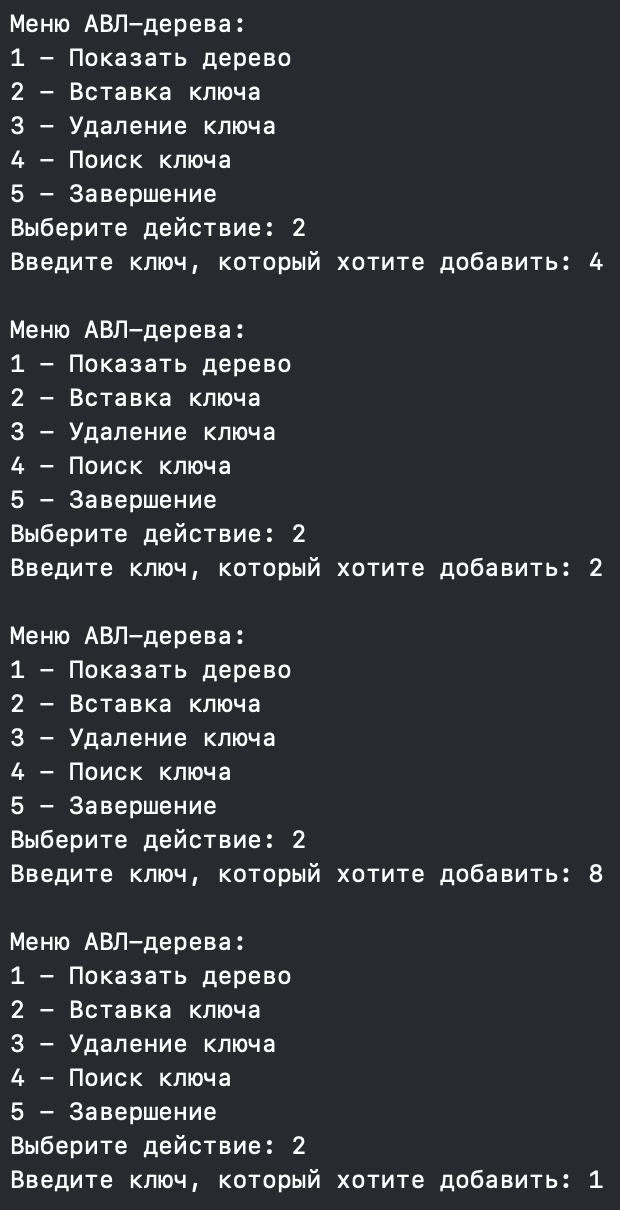
\includegraphics[scale=0.7]{ex1_1.png}}
  		\caption{Пример работы $1$}
  		\label{img:grap1}
	\end{figure}
	\newpage
	\begin{figure}[h]
  		\center{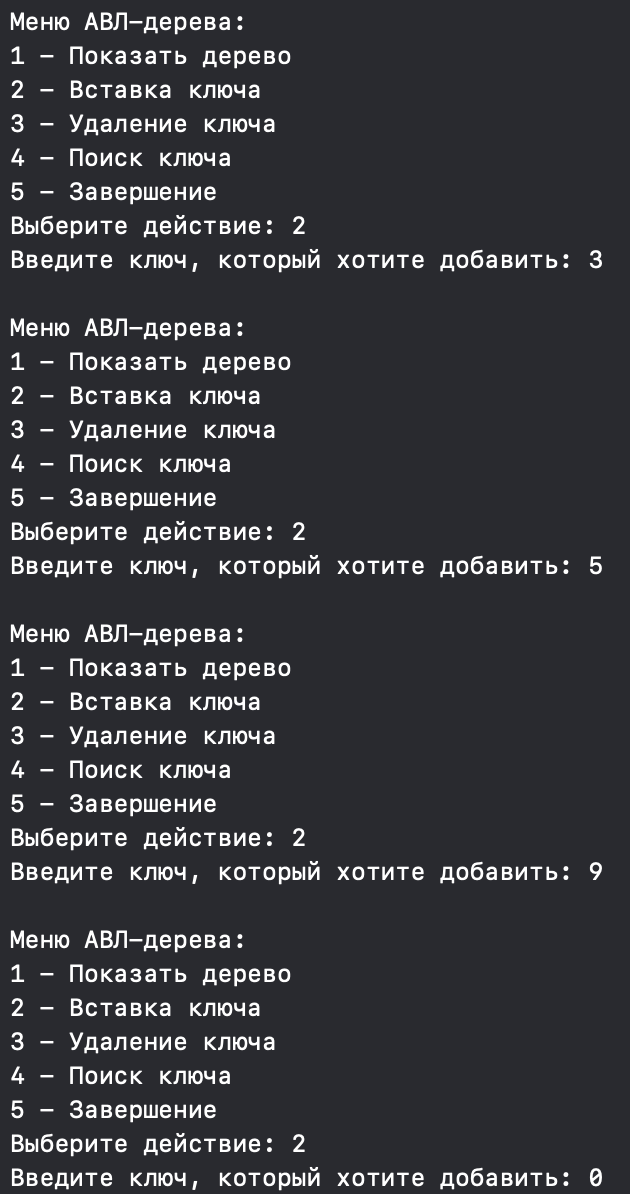
\includegraphics[scale=0.7]{ex1_2.png}}
  		\caption{Пример работы $2$}
	\end{figure}
	\newpage
	\begin{figure}[h]
  		\center{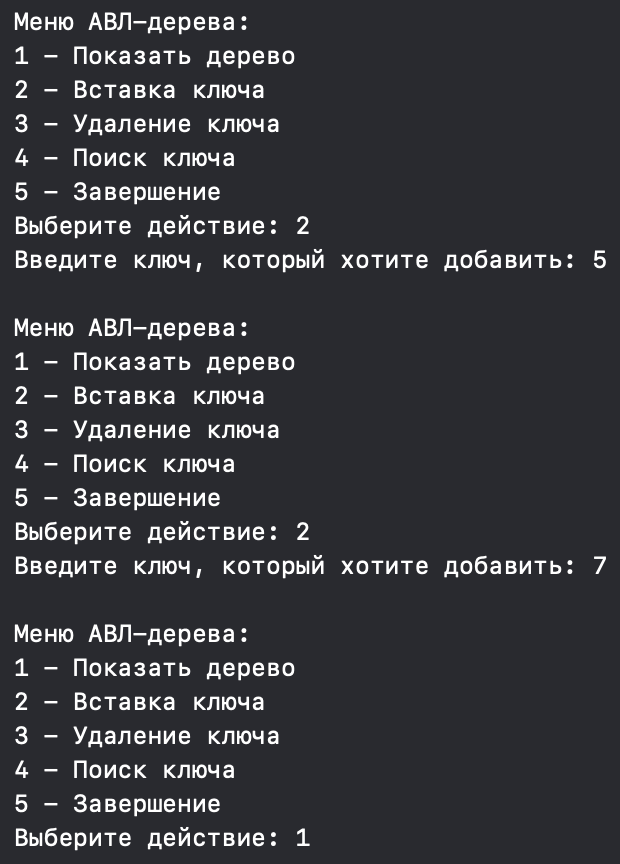
\includegraphics[scale=0.7]{ex1_3.png}}
  		\caption{Пример работы $3$}
	\end{figure}
	\newpage
	\begin{figure}[h]
  		\center{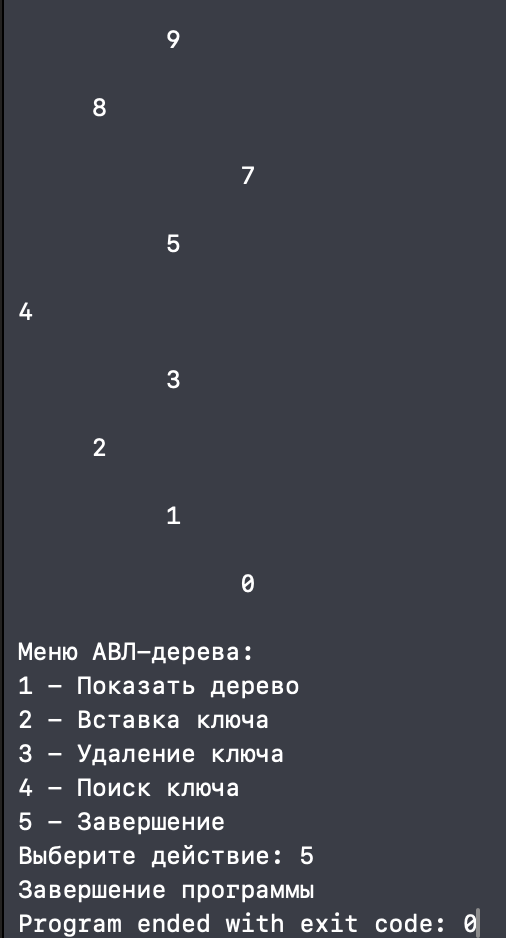
\includegraphics[scale=0.7]{ex1_4.png}}
  		\caption{Пример работы $4$}
	\end{figure}
	\newpage
\end{enumerate}
\newpage
\section*{Заключение}
\addcontentsline{toc}{section}{Заключение}
Цель достигнута, описана структура данных АВЛ-дерева. В результате 
выполнения лабораторной работы были выполнены все задачи.
\begin{enumerate}
\item Описаны алгоритмы добавления и удаления 
элемента, поиска элемента в дереве, балансировки дерева.
\item Разработана программу, предоставляющая пользователю выбор пункта 
меню, отображающая меню в цикле с постусловием, реализующая все описанные 
алгоритмы.
\item Приведены примеры работы программы.
\end{enumerate}
\newpage
\begin{center}
\begin{thebibliography}{}
\addcontentsline{toc}{section}{Список используемых источников}
\bibitem{book}Матвеева. Т.К., Балансировка при включении в AVL дерево: 
Методическая разработка 2013. – 13 с.
\end{thebibliography}
\end{center}
\end{document}
